\documentclass{article}

\usepackage{PRIMEarxiv}

\usepackage[utf8]{inputenc} % allow utf-8 input
\usepackage[T1]{fontenc}    % use 8-bit T1 fonts
\usepackage{hyperref}       % hyperlinks
\usepackage{url}            % simple URL typesetting
\usepackage{booktabs}       % professional-quality tables
\usepackage{amsfonts}       % blackboard math symbols
\usepackage{nicefrac}       % compact symbols for 1/2, etc.
\usepackage{microtype}      % microtypography
\usepackage{fancyhdr}       % header
\usepackage{graphicx}       % graphics
\usepackage{amsmath,amssymb,amsthm,xcolor,enumitem,caption,float,needspace,array,multirow}
\usepackage{tikz}
% generated by `python experiments.py` -- do not edit by hand
\newcommand{\PoaRandom}{1.3--3.2}
\newcommand{\PoaRandomExp}{1.1--2.7}
\newcommand{\LostRoad}{11.9}
\newcommand{\LostMess}{1.5}
\newcommand{\HoursFluid}{132}
\newcommand{\HoursRandom}{99}
\newcommand{\EightBetter}{52}
\newcommand{\EightWith}{56}
\newcommand{\EightFade}{2\%}
\newcommand{\EightMixed}{1.35}
\newcommand{\EightBestGap}{60\%}
\newcommand{\CERange}{0.5--1.8}
\newcommand{\RwThreeMzero}{0.7--2.8}
\newcommand{\RwThreeMtwo}{0.13--0.32}
\newcommand{\RwOneMtwo}{0.33--1.29}
\newcommand{\OptRange}{0.13--0.31}
\newcommand{\BackfireClear}{3}
\newcommand{\BackfireMarginal}{1}
\newcommand{\BackfireList}{road (+40\%), gym (+18\%), mess (+23\%)}
\newcommand{\BackfireMarginalList}{food court (+1\%)}
\newcommand{\RoadP}{probability 0.1: +3\%, probability 0.3: +20\%, probability 0.5: +30\%}
\newcommand{\PrivMax}{0.8\%}
\newcommand{\MessFiftyNobody}{10.9}
\newcommand{\MessFiftyAnn}{13.5}
\newcommand{\MessFiftyHint}{10.4}
\newcommand{\RunMinutes}{25}
\newcommand{\NoisySeeds}{10}
\newcommand{\TestsSig}{15}
\newcommand{\TestsAll}{15}
\newcommand{\TestsMaxP}{0.011}
\newcommand{\VarCount}{8}
\newcommand{\VarSizes}{9}
\newcommand{\VarMixedMin}{6\%}
\newcommand{\VarMixedMax}{72\%}
\newcommand{\ChecksPass}{9}
\newcommand{\ChecksAll}{9}
\newcommand{\VarBeat}{7}
\newcommand{\PrivSmallSeventy}{2--11\%}
\newcommand{\PrivSmallFifty}{6--15\%}
\newcommand{\PrivSmallMax}{15\%}
\newcommand{\PrivLimitSeventy}{0.02\%}
\newcommand{\PrivLimitFifty}{5.7\%}
  % numbers quoted in the text, written by experiments.py
\usetikzlibrary{positioning,arrows.meta,fit}
\hypersetup{colorlinks=true,linkcolor=blue!50!black,citecolor=blue!50!black,urlcolor=blue!50!black}
% figures: ../results/figures/ (made by experiments.py), photos: ../docs/img/ (credits in Fig. 1)
\graphicspath{{../results/figures/}{../docs/img/}{./}{media/}}

% spacing: give equations, floats, tables and lists room to breathe
\makeatletter
\g@addto@macro\normalsize{%
  \setlength\abovedisplayskip{9pt plus 2pt minus 2pt}%
  \setlength\belowdisplayskip{9pt plus 2pt minus 2pt}%
  \setlength\abovedisplayshortskip{5pt plus 2pt}%
  \setlength\belowdisplayshortskip{6pt plus 2pt minus 1pt}}
\makeatother
\setlength{\textfloatsep}{14pt plus 3pt minus 3pt}
\setlength{\floatsep}{12pt plus 2pt minus 2pt}
\setlength{\intextsep}{12pt plus 2pt minus 2pt}
\renewcommand{\arraystretch}{1.15}
\setlist{itemsep=2pt,topsep=4pt,leftmargin=*}
\captionsetup{font=small,labelfont=bf,skip=6pt}
\newtheorem{proposition}{Proposition}

% colours shared with the figures, the website and the lab
\definecolor{cNE}{HTML}{EB6834}
\definecolor{cOPT}{HTML}{1BAF7A}
\definecolor{cCE}{HTML}{2A78D6}
\definecolor{cGOLD}{HTML}{EDA100}
\definecolor{cMUT}{HTML}{6F6B63}
\newcommand{\finding}[1]{\par\smallskip\noindent\colorbox{cCE!7}{\parbox{\dimexpr\linewidth-2\fboxsep}{\small\textbf{Finding.} #1}}\par\smallskip}

%Header
\pagestyle{fancy}
\thispagestyle{empty}
\fancyhead{}
\fancyhead[C]{Who Should Be Told What? Coordinating Crowds with Correlated Equilibrium}

\renewcommand{\undertitle}{Final Report \;|\; Foundations of AI -- Multi-Agent Systems \;|\; IIT Gandhinagar}

%% Title
\title{Who Should Be Told What? Coordinating Crowds at Shared Facilities with Correlated Equilibrium
\thanks{\textit{\underline{Source code}}: \url{https://github.com/YashG1836/crowd-congestion};
\textit{\underline{website}}: \url{https://yashg1836.github.io/crowd-congestion/};
\textit{\underline{interactive lab}}: \url{https://crowd-congestion.streamlit.app/}.
Every figure and number in this report is produced by \texttt{python experiments.py}. All data are synthetic.}}

\author{
  Harsh Kumar Jha \;(24110130)\\
  \normalfont Artificial Intelligence\\
  \normalfont\texttt{harsh.jha@iitgn.ac.in}
  \And
  Yash Goyal \;(24110399)\\
  \normalfont Computer Science and Engineering\\
  \normalfont\texttt{yash.g@iitgn.ac.in}
  \AND
  Piyush Kumar Keshri \;(24110260)\\
  \normalfont Chemical Engineering\\
  \normalfont\texttt{piyush.keshri@iitgn.ac.in}
  \And
  Garv Singhal \;(24110119)\\
  \normalfont Computer Science and Engineering\\
  \normalfont\texttt{garv.singhal@iitgn.ac.in}
}
\date{}

\begin{document}
\raggedbottom
\maketitle

\begin{figure}[H]\vspace{-4pt}\centering
\begin{tabular}{@{}c@{\hspace{5pt}}c@{\hspace{5pt}}c@{\hspace{5pt}}c@{}}
\includegraphics[width=0.2405\linewidth]{road.jpg} & \includegraphics[width=0.2405\linewidth]{canteen.jpg} &
\includegraphics[width=0.2405\linewidth]{network.jpg} & \includegraphics[width=0.2405\linewidth]{gym.jpg}\\[-1pt]
\small Roads: the morning rush & \small Canteens: the lunch queue & \small Networks: jobs on one link & \small Gyms: the after-work crowd
\end{tabular}
\caption{One problem in many places: a crowd, a bottleneck and a clock. Photos via Wikimedia Commons: Countryball
mys123 (CC BY 4.0), Freooudzao (CC BY-SA 4.0), BalticServers.com (CC BY-SA 3.0), U.S.\ Air Force / Staff Sgt.\
Araceli Alarcon (public domain).}\label{fig:photos}
\end{figure}

\begin{abstract}
\noindent Many people share one bottleneck and each chooses \emph{when} to use it: cars at a bridge, backups on a
network link, diners at a food court, members at a gym, students at a hostel mess. We model this as a game of time
slots and a first-come-first-served queue. Selfish timing (the \emph{Nash equilibrium}) costs 3.3--8.0 times the
planner's schedule in five facilities (\PoaRandom{} times if arrivals inside a slot are random), and a public crowd display
that everyone reacts to multiplies the cost up to 17 times. Our main tool is the \emph{correlated equilibrium} (CE):
advice that people want to follow. Solving small crowds exactly, we show that the best CE beats every pure Nash
equilibrium (closing \EightBestGap{} of the gap to the planner at 10 people) and that the advantage fades as the crowd grows,
as our Proposition~2 predicts. Private advice drawn from a Nash schedule is obeyed by rational users and ends herding,
but noisy users drift away from it, because a Nash schedule leaves them nearly indifferent. The CE obedience
constraints price the smallest reward that makes the planner's schedule self-enforcing; a margin of 1--2 minutes
makes it hold for noisy users too. On bad days, \emph{what} is said matters most: announcing backfires on severe ones
in \BackfireClear{} of the five facilities (and barely in one more), while a calibrated hint never does worse; privacy
adds up to \PrivSmallMax{} in small crowds but little in large ones. We apply all of this to the four messes of IIT Gandhinagar (393,747 synthetic QR scans).
\end{abstract}

\keywords{Crowd congestion \and Nash equilibrium \and Correlated equilibrium \and Information design \and Price of anarchy}

% ============================================================================
\section{Introduction: everyone comes at once}

On a normal evening the IITGN mess is packed between 20:00 and 20:30 and nearly empty after 21:00, although its
counter could serve every student over the two hours. A toll plaza at 8:30, a network link when every laptop starts
its backup at 22:00, a food court at 13:00 and a gym after work look the same (Fig.~\ref{fig:photos}). Many people
share one bottleneck; each one chooses when to use it, wanting a convenient time and a short queue; and every person
who joins a queue delays everyone behind them while feeling only their own wait. Congestion here is a
\emph{coordination} problem, not a capacity problem.

The obvious fix is information. The mess already scans every plate with a QR code, so a live crowd counter is cheap.
But people who react to the same numbers move together: if the screen says that 20:10 is quiet, 20:10 becomes the
rush, as in Arthur's El Farol bar~\cite{arthur}. So the question of this project is:
\begin{center}\emph{What should be told to whom, so that people's own choices lead to short queues?}\end{center}

We answer it with two ideas from game theory. The \textbf{Nash equilibrium}~\cite{nash} describes where selfish
timing settles, and so how much time is lost. The \textbf{correlated equilibrium}~\cite{aumann} describes advice that
people want to follow: a mediator (here an app) privately recommends a slot to each person, and nobody gains by
disobeying. A traffic light is the everyday example. We study the problem in general, on five facilities with one
model, and then apply it to the four messes of IIT Gandhinagar with eight weeks of synthetic QR-scan data.
Figure~\ref{fig:story} is the map of the report.

\begin{figure}[t]\centering
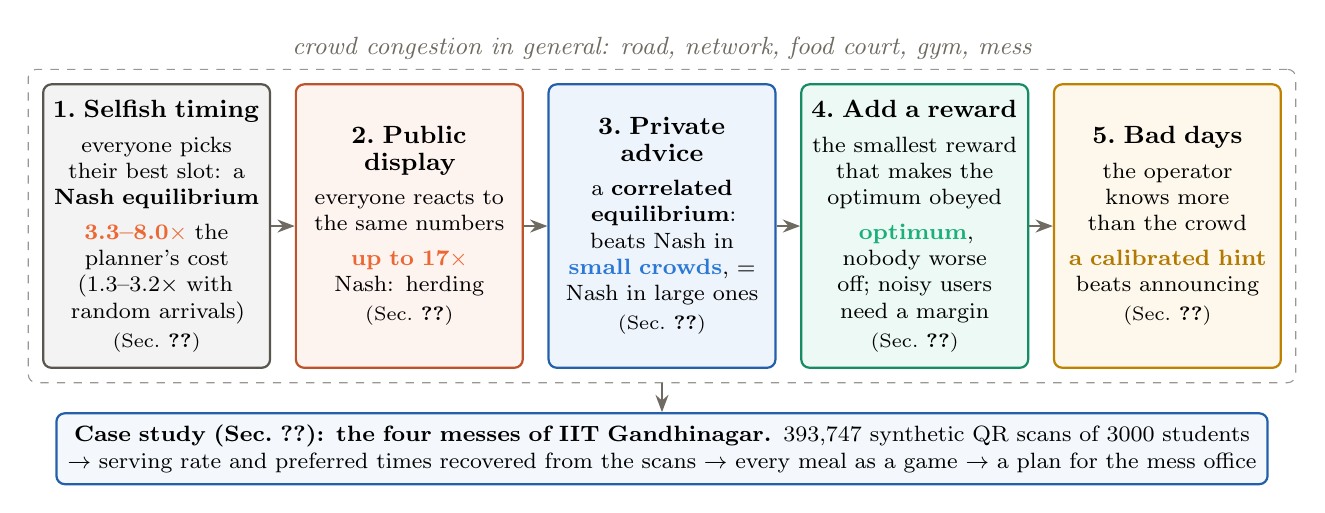
\begin{tikzpicture}[
  box/.style={draw=#1!80!black, fill=#1!8, rounded corners=3pt, line width=0.8pt, text width=2.6cm, minimum height=3.6cm,
              align=center, inner sep=4pt, font=\footnotesize, execute at begin node={\hyphenpenalty=10000\exhyphenpenalty=10000}},
  arr/.style={-{Stealth[length=2.2mm]}, line width=0.8pt, cMUT}]
\node[box=cMUT] (a) {{\small\bfseries 1.\ Selfish timing}\\[3pt] everyone picks their best slot: a \textbf{Nash equilibrium}\\[3pt] {\color{cNE}\textbf{3.3--8.0$\times$}} the planner's cost ({\PoaRandom$\times$} with random arrivals)\\[1pt]{\scriptsize (Sec.~\ref{sec:selfish})}};
\node[box=cNE, right=0.3cm of a] (b) {{\small\bfseries 2.\ Public display}\\[3pt] everyone reacts to the same numbers\\[3pt] {\color{cNE}\textbf{up to 17$\times$}} Nash: herding\\[1pt]{\scriptsize (Sec.~\ref{sec:display})}};
\node[box=cCE, right=0.3cm of b] (c) {{\small\bfseries 3.\ Private advice}\\[3pt] a \textbf{correlated equilibrium}: beats Nash in {\color{cCE}\textbf{small crowds}}, = Nash in large ones\\[1pt]{\scriptsize (Sec.~\ref{sec:ce})}};
\node[box=cOPT, right=0.3cm of c] (d) {{\small\bfseries 4.\ Add a reward}\\[3pt] the smallest reward that makes the optimum obeyed\\[3pt] {\color{cOPT}\textbf{optimum}}, nobody worse off; noisy users need a margin\\[1pt]{\scriptsize (Sec.~\ref{sec:reward})}};
\node[box=cGOLD, right=0.3cm of d] (e) {{\small\bfseries 5.\ Bad days}\\[3pt] the operator knows more than the crowd\\[3pt] {\color{cGOLD!75!black}\textbf{a calibrated hint}} beats announcing\\[1pt]{\scriptsize (Sec.~\ref{sec:bad})}};
\foreach \u/\v in {a/b,b/c,c/d,d/e} \draw[arr] (\u) -- (\v);
\node[draw=cMUT!70, dashed, rounded corners=3pt, fit=(a)(e), inner sep=5pt,
      label={[font=\small\itshape, text=cMUT]above:crowd congestion in general: road, network, food court, gym, mess}] (g) {};
\node[box=cCE, text width=15.1cm, minimum height=0.9cm, below=0.55cm of c, fill=cCE!5] (m) {\textbf{Case study (Sec.~\ref{sec:mess}): the four messes of IIT Gandhinagar.} 393{,}747 synthetic QR scans of 3000 students $\rightarrow$ serving rate and preferred times recovered from the scans $\rightarrow$ every meal as a game $\rightarrow$ a plan for the mess office};
\draw[arr] (g.south) -- (m.north);
\end{tikzpicture}
\caption{The story of this report. Each box is one step of the argument and its headline number.}\label{fig:story}
\end{figure}

\textbf{What we did.} (1)~One model and one set of solvers (Nash, optimum, large crowd, price of anarchy) for five
facilities (Sections~\ref{sec:model}--\ref{sec:selfish}). (2)~A day-to-day simulator of displays and crowds
(Section~\ref{sec:display}). (3)~Correlated advice end to end: exact small crowds that show when correlation beats Nash and how
the advantage fades, a proof that advice alone cannot beat Nash in a large crowd, a shuffled recommender, what happens
when its users are noisy, how many users it needs, the smallest reward that reaches the optimum, and whether learners
find a correlated equilibrium themselves (Section~\ref{sec:ce}). (4)~Who should be told what on bad days, including how
bad and how frequent they are (Section~\ref{sec:bad}). (5)~Robustness of the headline numbers to random arrivals
(Sections~\ref{sec:selfish} and~\ref{sec:bad}). (6)~The mess case study (Section~\ref{sec:mess}). (7)~A list of claims with their evidence and verification checks (Sections~\ref{sec:built}--\ref{sec:claims}). (8)~A tested library,
a website and an interactive lab (Section~\ref{sec:built}).

% ============================================================================
\section{The model: one game for every shared facility}\label{sec:model}
\textbf{People, slots and costs.} $n$ people share one bottleneck during $T=12$ slots of $\Delta$ minutes
(Table~\ref{tab:domains}). Person $i$ has a favourite slot $\tau_i$ and a flexibility $\beta_i$: the minutes of
waiting they would accept to avoid moving one slot (three levels: flexible, average, rigid). If $A_t$ people arrive in
slot $t$, the cost of person $i$ in slot $t$ is
\begin{equation}\label{eq:cost}
c_i(t) \;=\; W_t(A) \;+\; \beta_i\,|t-\tau_i| ,
\end{equation}
where $W_t$ is the average wait in slot $t$. The bottleneck serves $\mu$ people per minute, first come first served.
Arrivals spread evenly over their slot, someone who finds $q$ people ahead waits $q/\mu$ minutes, and the queue left
at the end of a slot carries over into the next one:
\begin{equation}\label{eq:queue}
Q_{t+1} \;=\; \max\bigl(0,\; Q_t + A_t - \mu\Delta\bigr).
\end{equation}
This is Vickrey's bottleneck model of a road~\cite{vickrey} and a buffer on a network link; between facilities only
the numbers change. The \emph{social cost} $SC$ is the sum of everyone's cost; we report it in minutes per person.
People with the same $(\tau,\beta)$ are interchangeable, so a schedule is a small table $X[k,t]$, the number of
people of type $k$ in slot $t$ (at most 36 types, even for 2400 cars).

\textbf{Nash equilibrium: selfish timing.} A schedule is a Nash equilibrium if nobody can lower their cost by moving
alone to another slot. We find it by best-response dynamics: repeatedly move the person who gains the most. Because the
queue carries over, the game has no potential function~\cite{rosenthal} and best response can cycle; we then return
the best $\varepsilon$-equilibrium seen and report $\varepsilon$, the largest gain any single person could still get
(at most 7\,s). Several starting schedules give several equilibria.

\textbf{The planner's optimum} is the schedule with the smallest $SC$. We solve a linear program on a one-minute grid
(arrivals and queue lengths are the variables and \eqref{eq:queue} the constraints), round it to whole people and
polish it by exact local search. The \textbf{price of anarchy} is $\mathrm{PoA}=SC(\text{worst Nash})/SC(\text{optimum})$~\cite{koutsoupias,roughgarden}.
In a \textbf{large crowd} each person is negligible and the equilibrium is a Wardrop equilibrium~\cite{wardrop}; we
compute it exactly (to within 0.02\,s) by projected extragradient~\cite{korpelevich} and use it where exactness matters
(Sections~\ref{sec:beat} and~\ref{sec:bad}).

\textbf{Correlated equilibrium.} A mediator draws a profile of recommendations $s=(s_1,\dots,s_n)$ from a
distribution $p$ and tells each person only their own $s_i$. The distribution $p$ is a \emph{correlated equilibrium}
(CE) if for every person $i$ and all slots $t,t'$
\begin{equation}\label{eq:ce}
\sum_{s:\;s_i=t} p(s)\,\bigl[c_i(s)-c_i(t',s_{-i})\bigr] \;\le\; 0 ,
\end{equation}
that is, a person who is told $t$, and knows nothing else, expects no gain from going to $t'$ instead. Every Nash
equilibrium is a CE ($p$ puts all its weight on it). The conditions are linear in $p$, so the best CE is a linear
program.

\begin{table}[t]\centering\small
\caption{Five shared facilities, one model. Selfish = the \emph{worst} Nash equilibrium found (the one in the price of
anarchy); planner = the optimum. Minutes per person per visit. PoA, random: the same two schedules when arrival times
inside each slot are random (Section~\ref{sec:selfish}). The last column is the ``bad day'' of Section~\ref{sec:bad}.}\label{tab:domains}
\setlength{\tabcolsep}{4pt}
\begin{tabular}{@{}lrrrrrrrl@{}}\toprule
Facility & People & Slot & $\mu$/min & Selfish & Planner & PoA & PoA, random & Bad day (70\% capacity)\\\midrule
Road: bridge commute & 2400 cars & 15\,min & 15 & 17.12 & 4.50 & 3.8 & 3.2 & a lane closed\\
Network: night backups & 600 jobs & 10\,min & 7 & 3.71 & 1.13 & 3.3 & 1.8 & link degraded\\
Food court: lunch & 450 diners & 10\,min & 6 & 2.35 & 0.50 & 4.7 & 2.2 & a counter closed\\
Gym: after work & 240 members & 20\,min & 1.5 & 1.68 & 0.31 & 5.4 & 1.3 & machines down\\
Mess: dinner (generic) & 680 students & 10\,min & 9 & 2.21 & 0.28 & 8.0 & 2.8 & staff short\\\bottomrule
\end{tabular}
\end{table}

% ============================================================================
\section{Step 1: selfish timing wastes time}\label{sec:selfish}
In every facility selfish timing costs 3.3--8.0 times the planner's schedule (Table~\ref{tab:domains},
Fig.~\ref{fig:selfish}): 17.1 against 4.5 minutes per car on the road, 2.2 against 0.28 minutes per student at the
mess. Almost all of the selfish cost is waiting (14.0 of the 17.1 minutes on the road). The planner removes the queue
almost entirely by feeding arrivals at exactly the service rate, at the price of moving some people one or two slots
away from their favourite time. The reason is the externality: a car that joins the 8:30 queue delays every car
behind it, but its driver counts only their own wait. The bumpy Nash profile in Fig.~\ref{fig:selfish} is real, not
noise: the slot right after a rush inherits its queue, so arriving at the start of a rush is better than just after it.

\textbf{How much of this is the fluid queue?} The planner's zero wait comes from spreading arrivals perfectly evenly
inside each slot. Real arrivals bunch up. We therefore keep the two schedules but draw every arrival time at random
inside its slot, serve people one at a time at rate $\mu$ and measure the waiting by simulation (200 runs). The
planner now waits too, and the price of anarchy falls to \PoaRandom{} (\PoaRandomExp{} if service times are also random;
Table~\ref{tab:domains}, Fig.~\ref{fig:robust} left). Selfish timing still costs \LostRoad{} minutes per car and \LostMess{} per student. The ratios in the rest of the report use the fluid model and should be read as upper
bounds; the minutes lost and the comparisons between policies are what matter.

\begin{figure}[t]\centering\includegraphics[width=\linewidth]{fig2_selfish_vs_planner.png}
\caption{Left: minutes lost per person under selfish timing and under the planner (labels: price of anarchy). Right:
the morning commute. Selfish drivers (orange) overload the bridge around 8:30; the planner (green) feeds it at
capacity.}\label{fig:selfish}\end{figure}

% ============================================================================
\section{Step 2: a public display can make things worse}\label{sec:display}
\textbf{Simulator.} The same people choose a slot every day for 150 days (the first 50 are discarded; 30 random seeds;
95\% confidence intervals are within 6\% of the mean). Policies are compared on the same seeds, so differences are
tested with two-sided paired sign-flip permutation tests and Holm's correction within each family of
comparisons~\cite{holm}: \TestsSig{} of the \TestsAll{} comparisons behind Sections~\ref{sec:display}
and~\ref{sec:reward} are significant at 5\% (largest adjusted $p$ = \TestsMaxP). Each day some people reconsider. Such a person picks slot $t$
with probability proportional to $e^{-\lambda\,\hat c_i(t)}$, where $\hat c_i(t)$ is the cost they expect in $t$
from what they are shown plus their inconvenience (logit choice~\cite{mckelvey}); everyone else keeps yesterday's
slot. We use three crowds: \emph{calm} ($\lambda=3$, 30\% reconsider each day), \emph{reactive} ($\lambda=3$,
everyone reconsiders) and \emph{noisy} ($\lambda=1$, 30\%). The policies are: \emph{no information} (people remember
only the waits of slots they visited), a \emph{public display} of yesterday's wait in every slot, the same display
seen by only 30\% of people, and three kinds of private advice that we study in Section~\ref{sec:ce}.

\textbf{Results} (Fig.~\ref{fig:display}). With a reactive crowd the public display multiplies the cost 3.7--17
times compared with Nash, and 75--89\% of people change slot every day: yesterday's quiet slot is today's rush (the
stripes in Fig.~\ref{fig:dinners}). Showing the same display to only 30\% of people removes almost all of the damage
(0.82--1.35$\times$ Nash), because too few people move together to shift the rush. With a calm crowd the display costs
at most 2.2$\times$ Nash. ``No information'' looks good (0.71--1.11$\times$ Nash), but only because people who
remember only the slots they visited stay pessimistic about the others; their regret (up to 3.9 minutes a day) shows
that this would not last once they learned.

\finding{Information that everyone reacts to in the same way creates herding. The cure is either fewer viewers or
advice that differs between people, which is where the correlated equilibrium comes in.}

\begin{figure}[t]\centering\includegraphics[width=\linewidth]{fig3_public_display.png}
\caption{Cost of each information policy relative to the Nash equilibrium (1 = Nash; log scale), for five facilities
and three crowds. The public display (orange) is harmful for a reactive crowd. Here app users are rational (they disobey only if it
saves more than 6\,s), so CE advice (blue) is exactly Nash by construction; Section~\ref{sec:stable} lets them be as
noisy as everyone else. Only CE advice with a reward (green) gets close to the optimum.}\label{fig:display}\end{figure}

% ============================================================================
\section{Step 3: correlated equilibrium, advice that people want to follow}\label{sec:ce}
\subsection{In small games correlation can beat every Nash equilibrium}\label{sec:small}
\textbf{Two students, Peak or Late.} The popular slot (Peak) costs the number of students there (1 or 2); Late
always costs 1.5. In a pure Nash equilibrium one student goes Peak and the other Late, which is optimal (total 2.5),
but somebody has to volunteer for Late. Without coordination the symmetric equilibrium is mixed: each goes Peak with
probability $\nicefrac{1}{2}$, total 3.0. A shared counter that both react to makes them alternate between ``both
Peak'' and ``both Late'', total 3.5: herding in miniature. A \emph{private fair coin} that tells one student Peak and
the other Late is a correlated equilibrium: a student told Late knows the other was told Peak, so switching would cost
2 instead of 1.5. It reaches the optimum (2.5) and is fair, since each student is told Peak half the time
(Fig.~\ref{fig:small}, left). This coin only mixes the two pure Nash equilibria, so a public coin would do the same:
it shows coordination, not something beyond Nash.

\textbf{A traffic light.} Two drivers choose Stop or Go: both stop 6/6, one goes 7/2, both go 0/0 (a crash; here
higher is better). The best CE, from the linear program~\eqref{eq:ce}, says ``both stop'' with probability
$\nicefrac12$ and ``one goes'' with $\nicefrac14$ each. It never causes a crash and gives each driver 5.25, more than
any symmetric Nash outcome (4.67). Here privacy matters: ``both stop'' is not a Nash equilibrium, and a driver told
Stop obeys only because they do not know whether the other was told Stop or Go.

\begin{figure}[t]\centering\includegraphics[width=\linewidth]{fig1_small_games.png}
\caption{Small games. Left: the two-student game under three kinds of information. Middle: the traffic light: the best
correlated equilibrium never produces a crash. Right: learners find equilibria on their own (Section~\ref{sec:learn}).}\label{fig:small}\end{figure}

\subsection{From two people to a crowd: the shuffled recommender}\label{sec:rec}
The app picks a schedule $X$. Every day, inside each type, a random shuffle decides who is told which slot, so a
type-$k$ person is told slot $t$ with probability $X[k,t]/n_k$ and inconvenient slots rotate between similar people.

\begin{proposition}[Shuffled Nash advice is a correlated equilibrium]\label{p1}
If $X$ is a Nash equilibrium, the shuffled recommendation is a correlated equilibrium.\end{proposition}
\noindent\emph{Proof.} Whatever the shuffle, every type's slot counts are those of $X$. A person told $t$ therefore
knows the loads exactly, and since $X$ is a Nash equilibrium, $t$ is a best response for their type.\qed

\smallskip
In all five facilities the largest gain from disobeying CE advice is the equilibrium's own accuracy (0--6\,s). The
planner's optimum, used as advice, is \emph{not} a CE. The people it sends away from the peak (11--56\% of them) would
gain up to 2.9--18 minutes by going to the peak instead, and when they do, the cost rises \emph{above} Nash
(1.3--4.8$\times$, pink bars in Fig.~\ref{fig:display}).

\subsection{From two people to a crowd, solved exactly}\label{sec:exact}
Between two drivers and 2400 cars exactness is usually lost: the CE linear program has one variable per profile, $3^n$
of them for $n$ people and three slots. For identical people we do not need them. Relabelling identical people keeps a
CE a CE at the same cost, so averaging any CE over all relabellings gives one of the form ``draw a schedule $X$, then
shuffle'', and the linear program over all \emph{schedules} gives the exact best CE (we check it against the full
program over all $3^6$ profiles). We take $n$ identical people, three 10-minute slots, everyone preferring the middle
one ($\beta=2$), and a bottleneck that grows with the crowd (load 0.8), so that only the weight of one person changes
with $n$. Every number in Fig.~\ref{fig:exact} (left) is exact.

The best CE is strictly cheaper than every pure Nash equilibrium in \EightBetter{} of the \EightWith{} crowd sizes from 2 to 60 that
have one. At 10 people it costs 1.56 minutes against 2.12 for the only pure Nash equilibrium (planner 1.20): it closes
60\% of the gap. On 99\% of days it sends one more person to the late slot than the Nash equilibrium does (4/5/1
instead of 4/6/0). That person would gain 4 seconds by returning to the peak, but cannot tell this day from the rare
day (1\%) on which the advice is 8/0/2: then the peak inherits a long queue from the crowded early slot and returning
would cost over 3 minutes. Weighted by how often each happens, obeying is a best response. This is exactly what a correlated equilibrium can do and a Nash equilibrium cannot. The advantage fades
as one person's weight shrinks: at 51--60 people the best CE closes only \EightFade{} of the gap, which is
Proposition~\ref{p2} below seen directly. At 7, 9 and 11 people there is no pure Nash equilibrium at all, while a CE
always exists. Finally, a pure Nash equilibrium tells identical people who should go where, which they cannot agree on
alone; without any coordination they play the symmetric mixed equilibrium, which costs 3.02 minutes at 10 people and is
still \EightMixed{} times the best CE at 60. So even where advice cannot beat the best Nash equilibrium, it is what makes that
equilibrium reachable.

\textbf{Other crowds.} Table~\ref{tab:variants} repeats the exact analysis for \VarCount{} crowds of different shapes
(\VarSizes{} sizes from 4 to 40 each). Three things hold in every one of them: a CE exists, it is never worse than
the best pure Nash equilibrium, and it is far cheaper than uncoordinated play (by \VarMixedMin{} to \VarMixedMax{}
where the mixed equilibrium can be computed). Pure Nash equilibria often do not exist at all: with four slots or at full
load, at most sizes. Beating the \emph{best} pure Nash equilibrium happens in \VarBeat{} of the \VarCount{} crowds, but
not at every size (for example at 3 of 9 sizes when people are rigid). The precise claim is therefore: correlation
always beats uncoordinated play, often beats the best equilibrium, and never does worse.

\begin{table}[t]\centering\small
\caption{Small crowds of other shapes, solved exactly (crowd sizes 4, 6, 8, 10, 12, 16, 20, 30, 40). Pure Nash exists:
sizes at which there is a pure Nash equilibrium. CE beats it: sizes at which the best CE is strictly cheaper than every
pure Nash equilibrium. Largest saving: of the best CE over the best pure Nash. Versus mixed Nash: saving over the
symmetric mixed equilibrium (one-type crowds only).}\label{tab:variants}
\begin{tabular}{@{}lrrrr@{}}\toprule
Crowd & pure Nash exists & CE beats it & largest saving & versus mixed Nash\\\midrule
\csname @@input\endcsname generated/tab_variants.tex 
\bottomrule\end{tabular}\end{table}

\begin{figure}[t]\centering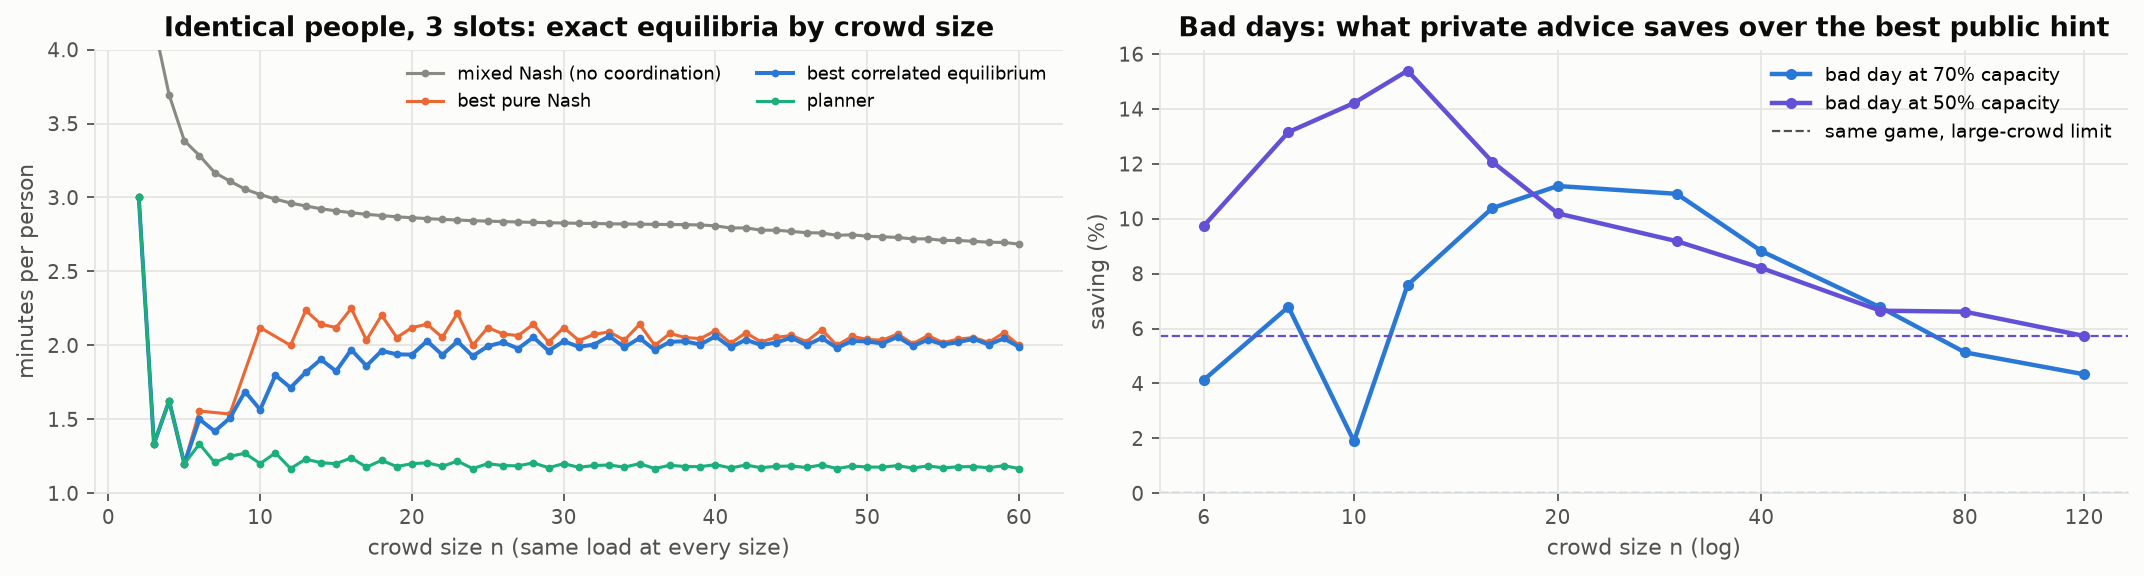
\includegraphics[width=\linewidth]{fig9_small_crowds.png}
\caption{Small crowds solved exactly (identical people, three slots). Left: cost per person by crowd size; the best
correlated equilibrium beats every pure Nash equilibrium and, by far, the uncoordinated mixed one, and the advantage over
pure Nash fades as the crowd grows. Right (Section~\ref{sec:bad}): on bad days, what private advice saves over the best
public hint; dashed lines are the same game in the large-crowd limit.}\label{fig:exact}\end{figure}

\subsection{Can advice alone beat Nash in a large crowd?}\label{sec:beat}
In small crowds correlation won because one person's choice changes the others' costs. In a large crowd each person
is negligible.

\begin{proposition}[Advice alone cannot beat Nash in a large crowd]\label{p2}
In a large crowd with complete information, if each slot's congestion cost depends only on that slot's load and
strictly increases with it, every coarse correlated equilibrium, and hence every CE, has the loads and the cost of the
Nash (Wardrop) equilibrium $x^*$.\end{proposition}
\noindent\emph{Proof sketch.} Compare each type's obedience with ``always go where $x^*$ sends you'' and add these
conditions with weights $x^*$. This gives $\sum_s p(s)\,\langle x^s-x^*,c(x^s)\rangle\le 0$, where $x^s$ is the
schedule of profile $s$ and $c(\cdot)$ the vector of costs. Each term splits into
$\langle x^s-x^*,\,c(x^s)-c(x^*)\rangle\ge0$ (costs increase with the load) plus $\langle x^s-x^*,\,c(x^*)\rangle\ge 0$
($x^*$ is an equilibrium), so both are zero, and strictly increasing costs force equal loads.\qed

\smallskip
Our queue carries over, so a slot's wait also depends on earlier slots and Proposition~\ref{p2} is \emph{not} a
theorem for our model. We check it numerically with the linear program~\eqref{eq:ce} over every randomisation of about
25 schedules (the Nash schedule, the optimum and schedules in between). Table~\ref{tab:ce} shows that in all five
facilities this best CE costs what Nash costs, both in the real (atomic) game, with the tolerance $\varepsilon$, and in
the large-crowd game. A menu cannot rule out a better CE elsewhere, so this supports the claim for our queue without
proving it; Section~\ref{sec:exact} showed the same fading exactly, for every crowd small enough to list.

\finding{Advice coordinates, but on its own it cannot ask anybody to take a worse slot for the common good.}

\begin{table}[t]\centering\small
\caption{Correlated advice in numbers. Nash = the \emph{best} Nash equilibrium found (Table~\ref{tab:domains} uses the
worst; they differ most in the gym, 1.44 against 1.68, which has several equilibria). Left: the best correlated
equilibrium found by the linear program equals Nash.
Right (Proposition~\ref{p3}): who is tempted by the optimum, the reward that removes the temptation, the time it saves,
and how many people end up worse off than under selfish timing. Minutes per person.}\label{tab:ce}
\begin{tabular}{@{}l|rr|rr|rrrr@{}}\toprule
 & \multicolumn{2}{c|}{real game} & \multicolumn{2}{c|}{large crowd (exact)} & \multicolumn{4}{c}{optimum + obedience reward}\\
Facility & Nash & best CE & Nash & best CE & tempted & reward & saving & worse off (no reward / reward)\\\midrule
Road & 16.98 & 16.98 & 17.09 & 17.09 & 52\% & 4.48 & 12.48 & 267 / 0\\
Network & 3.69 & 3.69 & 3.74 & 3.74 & 56\% & 1.09 & 2.56 & 0 / 0\\
Food court & 2.24 & 2.24 & 2.38 & 2.38 & 20\% & 0.48 & 1.75 & 0 / 0\\
Gym & 1.44 & 1.44 & 1.68 & 1.68 & 13\% & 0.27 & 1.14 & 10 / 0\\
Mess & 2.16 & 2.16 & 2.16 & 2.16 & 11\% & 0.27 & 1.88 & 0 / 0\\\bottomrule
\end{tabular}
\end{table}

\subsection{What advice is good for, and what happens when users are noisy}\label{sec:stable}
With rational app users, who disobey only if it saves more than 6 seconds, CE advice gives exactly the Nash cost for
every kind of crowd in every facility (blue bars in Fig.~\ref{fig:display}), with nobody switching slots: people obey
because it is in their own interest, from the first day. This is by construction, since the advice is a CE up to the
equilibrium's accuracy (at most 6\,s). The test is users who are as noisy as everyone else. Told slot $r$, such a user
picks slot $t$ with probability proportional to $e^{-\lambda c(t)}$, where $c(t)$ is what $t$ would cost them if the
others obey (the app can compute it), with $\lambda=3$ (as in the calm crowd) or $\lambda=1$ (the noisy crowd).
Table~\ref{tab:noisy} shows the result. CE advice is then no longer exactly Nash: \CERange{} times Nash, better where
random deviations happen to spread a rush and worse elsewhere. The reason is that a Nash schedule leaves people almost
indifferent between their slot and the next one (that is what equilibrium means in a crowd), so the advice gives them
only seconds of reason to obey. The reward of Proposition~\ref{p3} has the same knife edge, because it removes the
temptation exactly; we return to it in Section~\ref{sec:reward}.

\begin{table}[t]\centering\small
\caption{App users as noisy as everyone else: cost relative to Nash (1 = Nash). $\lambda$: how sharply users prefer
cheaper slots; margin: minutes of reward on top of Proposition~\ref{p3}'s, so that obeying is strictly better.
Last column: the planner (the best possible). \NoisySeeds{} seeds $\times$ 50 days.}\label{tab:noisy}
\begin{tabular}{@{}l|rr|rrr|rrr|r@{}}\toprule
 & \multicolumn{2}{c|}{CE advice} & \multicolumn{3}{c|}{CE advice + reward, $\lambda=3$} & \multicolumn{3}{c|}{CE advice + reward, $\lambda=1$} & \\
Facility & $\lambda=3$ & $\lambda=1$ & margin 0 & 1 & 2 & margin 0 & 1 & 2 & planner\\\midrule
\csname @@input\endcsname generated/tab_noisy.tex 
\bottomrule
\end{tabular}
\end{table}

CE advice also protects the people who do not use it (Fig.~\ref{fig:ceplot}, left). With a reactive crowd
and the public display for non-users, the cost falls from 3.7--17$\times$ Nash when nobody uses the app to within
10\% of Nash once 50--90\% of people use it (50\% is enough at the mess).

\subsection{The price of obedience: a reward that reaches the optimum}\label{sec:reward}
\begin{proposition}[Price of obedience]\label{p3}
For a schedule $X$ let $G[k,t]$ be the most that a type-$k$ person told $t$ could gain by moving alone (zero if
nothing is gained). A reward worth $G[k,t]$ minutes to the recipient for showing up in the recommended slot (for example a coupon) makes
the shuffled $X$ a correlated equilibrium of the rewarded game, and no smaller reward per slot does. The total reward is
$\sum_{k,t}X[k,t]\,G[k,t]$.\end{proposition}
\noindent\emph{Proof.} With the reward, staying costs at most what any move costs; with less, somebody still gains by
moving.\qed

\smallskip
Applied to the optimum (Table~\ref{tab:ce}, Fig.~\ref{fig:ceplot} right), the reward goes only to the people sent
away from the peak (11--56\%). It averages 0.27--4.48 minutes per person and saves 1.1--12.5 minutes per person: every
minute of reward saves 2.4--6.9 minutes of queueing. The reward is a transfer, not a loss, and with it nobody is worse
off than under selfish timing. Without it, the optimum already helps almost everyone (only 267 drivers and 10 gym members
would lose, by at most 3 minutes), yet it is not stable, because each person sent off-peak would gain even more by sneaking back. This
is the social dilemma that the reward resolves. The reward is a transfer from the operator, valued in minutes; turning it
into rupees needs a value of time. It should be something like a coupon: a priority token would not work, because at
the planner's schedule there is almost no queue to skip, and skipping a queue delays others. With noisy users
(Table~\ref{tab:noisy}) the exact reward leaves the planner's schedule as fragile as Nash (\RwThreeMzero{} times Nash at
$\lambda=3$). A margin of 2 minutes on top restores it (\RwThreeMtwo, against \OptRange{} for the planner), at a cost of 2 minutes per
person; very noisy users ($\lambda=1$) still get only part of the way (\RwOneMtwo).

\begin{figure}[t]\centering\includegraphics[width=\linewidth]{fig4_ce_advice.png}
\caption{Left: a reactive crowd in which only a share of people use CE advice and the rest see the public display.
Right: the price of obedience. The reward needed (with the share of people who receive one) is a fraction of the time
it saves.}\label{fig:ceplot}\end{figure}

\subsection{Can people find a correlated equilibrium without an app?}\label{sec:learn}
Regret matching~\cite{hart} (players move away from actions they regret) has no \emph{swap} regret, so the joint
play approaches the set of CEs. Hedge~\cite{freund} has no external regret and approaches the larger coarse-CE set.
EXP3~\cite{auer} learns from its own wait only. In the traffic light, regret matching ends 0.0045 from the CE set
after 6000 rounds (Fig.~\ref{fig:small}, right). In the five facilities, when every slot's wait is published,
regret-matching learners settle at 0.99--1.08$\times$ Nash (1.36$\times$ in the small gym) with a swap regret of at
most 0.45 minutes. EXP3 learners, who see only their own wait, still have 2.7--9.0 minutes of regret after 300 days.
Publishing every slot's wait helps people learn; an app gets them to the CE on the first day.

% ============================================================================
\section{Step 4: bad days, or who should be told what}\label{sec:bad}
On a \emph{bad day}, which happens with probability $p=0.3$, the bottleneck runs at 70\% of its capacity
(Table~\ref{tab:domains}, last column). The operator knows whether today is bad; the crowd knows only $p$. If
everyone believes ``bad with probability $q$'', they play the large-crowd equilibrium $x_q$ of the expected costs,
and the expected cost per person is
\begin{equation}\label{eq:V}
V(q) \;=\; (1-q)\,SC_{\text{normal}}(x_q) \;+\; q\,SC_{\text{bad}}(x_q).
\end{equation}
We compare five ways of using the operator's knowledge:
\begin{itemize}
\item \textbf{Tell nobody.} Everyone keeps the belief $p$ (a Bayesian Nash equilibrium~\cite{harsanyi}): cost $V(p)$.
\item \textbf{Announce the state.} Beliefs become 0 or 1: cost $(1-p)\,V(0)+p\,V(1)$.
\item \textbf{Best public hint.} A public message moves everyone's belief to some $q$, and on average the belief must
remain $p$. The best public signal therefore gives the lower convex envelope of $V$ at $p$ (Bayesian persuasion,
``concavification''~\cite{kamenica}); with two states, two messages (``quiet'' and ``busy'') are enough.
\item \textbf{Private advice.} The best \emph{Bayes correlated equilibrium}~\cite{bergemann}: recommendations may
depend on the state, and the obedience condition~\eqref{eq:ce} must hold on average over the days on which a given
piece of advice is sent. It is a linear program over 130 schedules.
\item \textbf{Planner, informed.} The optimum of each day (it needs the rewards of Section~\ref{sec:reward}).
\end{itemize}
Every public outcome is also a Bayes CE, so private advice is never worse than the best public hint. The question is
by how much.

\begin{table}[t]\centering\small
\caption{Who should be told what: expected cost per person (minutes) when a bad day (70\% capacity) happens with
probability 0.3. Large-crowd equilibria, accurate to 5\,s or better. Private advice is never worse than the best public hint.}\label{tab:bad}
\begin{tabular}{@{}lrrrrr|r@{}}\toprule
Facility & Tell nobody & Announce & Best public hint & Private advice & Hint: ``busy'' sent on bad / normal days & Planner\\\midrule
Road & 22.56 & \textcolor{cNE}{27.04} & 21.91 & 21.87 & 52\% / 18\% & 7.48\\
Network & 6.48 & 5.41 & 5.41 & 5.41 & 100\% / 0\% & 1.54\\
Food court & 5.36 & 3.90 & 3.90 & 3.89 & 100\% / 0\% & 0.89\\
Gym & 7.07 & 3.59 & 3.59 & 3.58 & 100\% / 0\% & 0.75\\
Mess & 4.25 & 3.19 & 3.13 & 3.13 & 100\% / 5\% & 0.62\\\bottomrule
\end{tabular}
\end{table}

\textbf{Results} (Table~\ref{tab:bad}, Fig.~\ref{fig:bad}). Announcing helps a lot at the network, the food court,
the gym and the mess (16--49\% lower expected cost), and there the best public hint is to announce, or nearly so. On
the road it backfires: announcing raises the expected cost by 20\% (22.6 to 27.0 minutes per car). Not knowing
whether a lane is closed makes drivers spread out, and that spread is better than the selfish one \emph{on both kinds
of day}: the fear works like a toll. Announcing ``all clear'' brings the 8:30 rush back (12.5 to 17.1 minutes on
normal days). The best hint is deliberately vague: say ``busy'' on 52\% of bad days and on 18\% of normal days, so
that drivers stay unsure (their belief becomes 0.20 or 0.55). It beats both silence and announcing. Private advice
adds at most 0.2\% (2.3 seconds per person), about the numerical tolerance of the equilibria. The informed planner
shows how much room is left (7.5 minutes on the road), and reaching it needs rewards.

\textbf{How bad, and how often?} One bad day at 70\% with probability 0.3 is a single setting, so we vary both
(Fig.~\ref{fig:robust}, right). On a mild bad day (85\%) announcing helps in every facility. On a severe one (50\%) it
backfires clearly in \BackfireClear{} of the five facilities, \BackfireList, and barely in \BackfireMarginalList.
On the road it backfires at every probability we tried (\RoadP). The calibrated hint is never worse than either. So the road result is not a one-off: the worse the bad day, the more often announcing it backfires, which fits the
explanation above (uncertainty keeps people spread out, and a blunt announcement throws that away).

\textbf{When does privacy pay?} In the five facilities private advice adds at most \PrivMax{} over the best public hint at
any severity. That is over a menu of 130 schedules, so it is a lower bound on what private advice could do. In the
small crowd of Section~\ref{sec:exact}, where the linear program covers every schedule (and a public hint is followed by
the best CE of the belief it creates), privacy saves \PrivSmallSeventy{} on a 70\% day and \PrivSmallFifty{} on a 50\% day for 6--120
people (Fig.~\ref{fig:exact}, right). In the large-crowd limit of the same game it saves \PrivLimitSeventy{} on the 70\% day, as in
the facilities, but still \PrivLimitFifty{} on the 50\% day.

\finding{\emph{What} is said matters most: announcing can backfire, and the worse the bad day the more often it does,
while a calibrated hint never does worse than silence or full disclosure. \emph{Saying it privately} pays in small
crowds and on severe days, and adds little in large crowds facing mild ones.}

\begin{figure}[t]\centering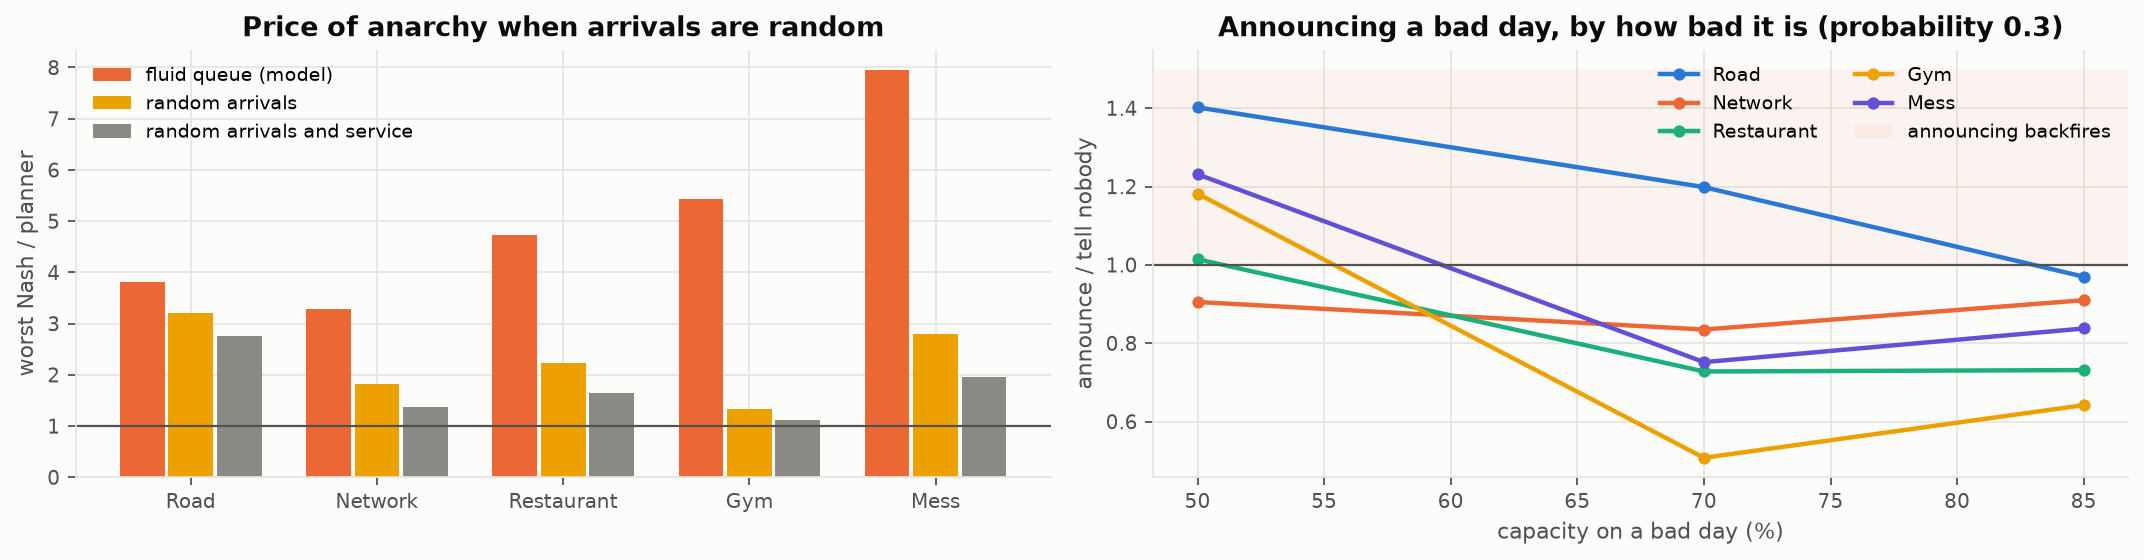
\includegraphics[width=\linewidth]{fig10_robustness.png}
\caption{Robustness. Left: price of anarchy with the fluid queue, with random arrival times inside each slot, and with
random service times as well (same schedules, 200 simulated runs). Right: announcing a bad day relative to telling
nobody, by how much capacity is left (probability 0.3); above the line announcing backfires.}\label{fig:robust}\end{figure}

\begin{figure}[t]\centering\includegraphics[width=\linewidth]{fig5_uncertainty.png}
\caption{Left: expected cost of each policy relative to telling nobody. Right: the road. The black curve is $V(q)$,
the cost when everyone believes ``bad day with probability $q$''. The best public hint is its lower convex envelope
(dashed) at the prior 0.3, and announcing is the dotted chord, which lies above silence.}\label{fig:bad}\end{figure}

% ============================================================================
\section{Case study: the IITGN mess}\label{sec:mess}
\subsection{The setting and the data}
IIT Gandhinagar has four messes (Jaiswal, Mohani, Argoras and Bhopal) for about 3000 students. Breakfast (from 07:30),
lunch (12:00) and dinner (19:30) last two hours each, which we split into 12 slots of 10 minutes; a counter serves 8
students per minute at breakfast and 9 at lunch and dinner. On a normal day 60\%, 85\% and 90\% of students come, with
a lunch rush after classes (around 13:05) and a dinner rush around 20:10. On special-menu days (Sunday breakfast and
lunch, Wednesday and Sunday dinner) 5\% more students come, the counter runs at 80\% speed and everyone comes 10 minutes
earlier. We simulate the status quo (no display; students choose by logit with memory) for eight weeks and write
exactly what the mess office would have: a QR-scan log (date, meal, mess, menu, student id, scan time), where the scan
time is the arrival time plus the exact queue wait. This gives \textbf{393,747 scans} (Fig.~\ref{fig:messdata}, left).
A hidden ground-truth table scores our estimates.

\begin{figure}[t]\centering\includegraphics[width=\linewidth]{fig6_mess_data.png}
\caption{Left: synthetic QR scans at the Jaiswal dinner, per 10 minutes and by weekday. The flat tops are the serving
rate; Wednesday and Sunday have special menus. Right: cost per student at every meal under selfish timing and under
the planner (average of the four messes).}\label{fig:messdata}\end{figure}

\subsection{What the scans reveal}
A scan happens when the plate is picked up, so waiting is not observed directly. Two facts are still easy to recover
(Table~\ref{tab:data}). \emph{The serving rate}: while a queue exists, plates leave at rate $\mu$, so the busiest
five minutes of scans estimate $\mu$ within 2--3\%. When no queue ever forms (a normal breakfast) this is only a lower
bound. \emph{Preferred times}: a student's median scan slot on normal days recovers their favourite slot exactly for
80--100\% of students, and within one slot for 97--100\%. This is all that the advice app of Section~\ref{sec:rec}
needs. Because the scans come from our own model, this shows that the estimators are consistent with it, not that they
would work on real logs; that needs the pilot of Section~\ref{sec:limits}. A short-term forecast of the next 30 minutes is accurate to 3.4--4.6 scans per slot (8--14\% of the load),
whether or not it is rescaled by tonight's first scans.

\begin{table}[t]\centering\small
\caption{Learning the unknowns from the scans alone. Serving rate: Jaiswal. Favourite slots: all 3000 students. Scans per
slot and forecast error (scans per slot, next 30 minutes, the better of two forecasters): average of the four messes.}\label{tab:data}
\begin{tabular}{@{}lrrrrr@{}}\toprule
Meal & true $\mu$ & estimated $\mu$ & favourite slot exact / within 1 & scans per slot & forecast error\\\midrule
Breakfast, normal / special & 8.0 / 6.4 & 6.2$^{\dagger}$ / 6.6 & 99.6\% / 100\% & 27.7 / 30.9 & 3.4 / 3.6\\
Lunch, normal / special & 9.0 / 7.2 & 9.2 / 7.4 & 91.3\% / 99.5\% & 39.5 / 41.6 & 4.0 / 3.4\\
Dinner, normal / special & 9.0 / 7.2 & 9.2 / 7.4 & 79.5\% / 96.9\% & 41.5 / 43.0 & 4.4 / 3.6\\\bottomrule
\multicolumn{6}{@{}l}{\footnotesize $^{\dagger}$No queue forms at a normal breakfast, so the scans give only a lower bound.}
\end{tabular}
\end{table}

\subsection{Every meal as a game}
Each mess, meal and menu is one game of Section~\ref{sec:model}, built from the roster (24 games). A normal dinner
loses 1.8 minutes per student to selfish timing and a special dinner 7.6 (Fig.~\ref{fig:messdata}, right); a normal
breakfast has no queue at all. Over the four messes and three meals of a normal day this adds up to \textbf{132
student-hours lost every day} with the fluid queue, and \HoursRandom{} when arrival times are random (Section~\ref{sec:selfish}).

\subsection{The Jaiswal dinner, day by day}
Figure~\ref{fig:dinners} replays 40 dinners of a reactive crowd, and Table~\ref{tab:jaiswal} compares every display
we considered. A public display of yesterday's queue raises the cost from 2.24 (Nash) to 11.55 minutes, and three
in four students change slot every evening. Making the display older (11.50) or coarser, as Low/Medium/High (12.95),
does not help, and private noise helps only partly (6.94): anything that everyone reacts to in the same way herds.
Two things do work: showing the display to at most half of the students (2.1 minutes, Fig.~\ref{fig:messdisplay}, left) or smoothing it into a moving-average forecast
(2.2). The display delay matters as well. With 30\% of students reacting each day, the daily swing grows from 2\% with
yesterday's numbers to 11\% with numbers four dinners old (Fig.~\ref{fig:messdisplay}, right): an old signal makes the
reaction overshoot. With rational students CE advice gives 2.24 minutes in every crowd with no swing at all, and with the obedience
reward the cost falls to \textbf{0.36} minutes, the planner's value (casual students need the margin of
Section~\ref{sec:reward}).

\begin{figure}[t]\centering\includegraphics[width=\linewidth]{fig7_mess_dinners.png}
\caption{Jaiswal dinner with a reactive crowd, dinners 51--90. Top: arrivals divided by the counter's capacity (red =
overload). Bottom: cost per student. The public display makes the rush jump around every evening; CE advice keeps a
steady schedule.}\label{fig:dinners}\end{figure}

\begin{table}[t]\centering\small
\caption{Every display policy at the Jaiswal dinner (minutes per student, 30 seeds; Nash 2.24, planner 0.36).}\label{tab:jaiswal}
\begin{tabular}{@{}lrrr|lrrr@{}}\toprule
Policy & calm & reactive & noisy & Policy & calm & reactive & noisy\\\midrule
No information & 1.65 & 2.11 & 1.84 & Display for 30\% of students & 2.02 & 2.10 & 1.89\\
Public display (yesterday) & 2.12 & \textcolor{cNE}{11.55} & 1.84 & Moving-average forecast & 2.17 & 2.20 & 1.88\\
Display, 3 dinners old & 4.07 & \textcolor{cNE}{11.50} & 2.73 & CE advice & 2.24 & 2.24 & 2.24\\
Display + private noise & 2.60 & \textcolor{cNE}{6.94} & 2.51 & Optimum as advice (no reward) & 3.61 & 3.61 & 3.61\\
Display in 3 levels & 3.83 & \textcolor{cNE}{12.95} & 3.34 & CE advice + reward & \textbf{0.36} & \textbf{0.36} & \textbf{0.36}\\\bottomrule
\end{tabular}
\end{table}

\begin{figure}[t]\centering\includegraphics[width=0.92\linewidth]{fig8_mess_display.png}
\caption{Showing information at the mess. Left: a reactive crowd when only a share of students see the display.
Right: the share of students who change slot every day, by display delay and by the share who reconsider each
day.}\label{fig:messdisplay}\end{figure}

\subsection{Who gains, and what to say on short-staffed days}
Coordination asks the flexible students to move, so it is fair to ask who pays. Under selfish timing students lose
2.1--2.3 minutes whatever their flexibility; those who like 20:00--20:30 lose 3.4 and the others 0.5. With the optimum and the reward, every group ends up
better off: flexible students, who are the ones asked to move and are paid for it, end with 0.03 minutes of net cost,
and rigid students with none. Without the reward 36 students would be worse off than under selfish timing, by at most
3 seconds. The reward costs 0.35 minutes per student on average. On a short-staffed evening (70\% speed, probability
0.3), announcing it lowers the expected cost from 4.47 to 3.47 minutes. On normal evenings it raises the cost (0.88 to
2.27), because the fear of a slow counter had been keeping students spread out. Unlike on the road, the net effect is
clearly positive, so the mess should announce a mild shortfall. A severe one is different: for the generic mess dinner
at 50\% speed, announcing raises the expected cost from \MessFiftyNobody{} to \MessFiftyAnn{} minutes, while a calibrated hint lowers it to
\MessFiftyHint.

\subsection{A plan for the mess office}
\begin{enumerate}
\item \textbf{Do not put yesterday's queue on a screen for everyone.} For a reactive crowd it multiplies the dinner
cost by five. If numbers are shown, show them to a few people or smooth them into a forecast.
\item \textbf{Send private slot suggestions drawn from a Nash schedule} (a small bot or app). Students who check them
obey without enforcement, the crowd stops swinging, and inconvenient slots rotate every day.
\item \textbf{Add a small reward for following the suggestion} (a dessert coupon, not a priority token) for the 13\% of
students sent off-peak, worth about 2.7 minutes each, plus a margin of 1--2 minutes' worth so that casual students
follow too. This takes the dinner from 2.24 towards 0.36 minutes per student.
\item \textbf{On mildly short-staffed evenings, tell students; on badly short-staffed ones, give a calibrated hint}
(``it may be slow tonight'') rather than a blunt announcement, which then backfires.
\item \textbf{Recalibrate weekly from the QR scans}: the serving rate from the busy stretches, the preferred times from
each student's usual scan time.
\end{enumerate}

% ============================================================================
\section{What we built}\label{sec:built}
\textbf{Library} (\texttt{crowd/}, Python with NumPy and SciPy/HiGHS): \texttt{game.py} (queue, game, Nash, optimum
and large-crowd solvers), \texttt{correlated.py} (recommender, obedience, CE linear programs, reward, who gains, bad-day
information design), \texttt{simulate.py} (simulator, displays, behaviour, learners), \texttt{domains.py} and
\texttt{mess.py} (facilities, mess scenario, scan generator, calibration), \texttt{theory.py} (small games),
\texttt{smallcrowd.py} (small crowds solved exactly: best CE, pure and mixed Nash, private and public advice).
\textbf{Checks} (Table~\ref{tab:checks}): \ChecksPass{} of \ChecksAll{} verification checks pass, and 72 unit tests, e.g.\ Pigou's 4/3 for linear costs, Proposition~\ref{p2} on the mess dinner, the
exact small-crowd CE against the full linear program over all profiles, the mixed equilibrium against support
enumeration, and ``private advice $\le$ best public hint $\le$ silence and announcing''. \textbf{Experiments}:
\texttt{python experiments.py} runs E1--E10 in about \RunMinutes{} minutes and writes every figure, the results and the website's
data.
\textbf{Website}: one page per step of the story with a 13-step automatic guided demo. \textbf{Interactive lab}: every
experiment live, for any facility or mess, with your own parameters (links on page 1).

% ============================================================================
\begin{table}[t]\centering\small
\caption{Verification checks, recomputed by every run of \texttt{experiments.py}.}\label{tab:checks}
\begin{tabular}{@{}>{\raggedright\arraybackslash}p{3.6cm}>{\raggedright\arraybackslash}p{6.2cm}>{\raggedright\arraybackslash}p{4.2cm}l@{}}\toprule
Check & What must hold & Result & Verdict\\\midrule
\csname @@input\endcsname generated/tab_checks.tex 
\bottomrule\end{tabular}\end{table}

\section{Claims and evidence}\label{sec:claims}
Table~\ref{tab:claims} lists every claim this report makes, the evidence for it and how far it holds.

\begin{table}[t]\centering\small
\caption{The claims of this report and the evidence for each.}\label{tab:claims}
\begin{tabular}{@{}l>{\raggedright\arraybackslash}p{4.6cm}>{\raggedright\arraybackslash}p{7.4cm}>{\raggedright\arraybackslash}p{2.2cm}@{}}\toprule
 & Claim & Evidence & Verdict\\\midrule
C1 & Selfish timing wastes time. & Price of anarchy 3.3--8.0 (fluid queue), \PoaRandom{} with random arrivals; \LostRoad{} minutes per car. & Holds; smaller with random arrivals\\
C2 & A display that everyone reacts to causes herding. & 3.7--17$\times$ Nash for a reactive crowd in all five facilities; 30\% viewers or private advice remove it (paired tests). & Holds for reactive crowds\\
C3 & Correlation beats Nash only when one person's move matters. & Exact small crowds: beats every pure Nash in \EightBetter{} of \EightWith{} sizes, fading to \EightFade{} at 51--60; never worse in \VarCount{} crowd shapes; Proposition~\ref{p2}; large-crowd LP = Nash. & Holds; not at every size\\
C4 & The obedience reward makes the planner's schedule self-enforcing. & Rational users: planner's cost, nobody worse off. Noisy users: \RwThreeMzero$\times$ Nash, \RwThreeMtwo$\times$ with a 2-minute margin. & Holds; needs a margin\\
C5 & Announcing a bad day can backfire. & Road +20\%; on severe days clearly in \BackfireClear{} facilities, barely in \BackfireMarginal; never on mild days; the calibrated hint never does worse. & Holds\\
C6 & Privacy matters in small crowds and on severe days. & Small crowds \PrivSmallSeventy{} (70\% day), \PrivSmallFifty{} (50\%); large-crowd limit \PrivLimitSeventy{} and \PrivLimitFifty; facilities at most \PrivMax{} over a menu. & Partly: facilities give only a lower bound\\
\bottomrule\end{tabular}\end{table}

\section{Limitations and future work}\label{sec:limits}
All data are synthetic, so the conclusions concern mechanisms (herding, obedience, the price of obedience, the value
of a hint) rather than exact IITGN minutes, and recovering parameters from our own scans shows consistency, not
validity. The fluid queue makes the planner look better than it is: with random arrivals the price of anarchy falls
from 3.3--8.0 to \PoaRandom{} (Section~\ref{sec:selfish}); we re-evaluated the schedules under randomness but did not
re-solve the equilibria for it. Proposition~\ref{p2} covers separable costs; for our queue it is checked over menus of
schedules, and exactly only for small identical crowds. The private-advice linear program for the five facilities
also uses a menu, so its small gain is a lower bound. Without a potential function we report $\varepsilon$-equilibria
(at most 7\,s). Behaviour models are assumptions: three crowds, and rational or logit app users. Next steps: a
Telegram-bot pilot in one mess with a second scan at the queue entrance to measure waiting directly; coupons as the
reward; and letting students choose between messes (a routing game, where Braess effects are possible).

% ============================================================================
\needspace{16\baselineskip}
\section{Contribution}
Four work packages, one per member, as in our project brief; all four of us shared the modelling, the analysis and
the writing.
\begin{table}[H]\centering\small
\caption{Work packages and status.}\label{tab:contrib}
\begin{tabular}{@{}>{\raggedright\arraybackslash}p{2.7cm}>{\raggedright\arraybackslash}p{11.5cm}>{\raggedright\arraybackslash}p{1.4cm}@{}}\toprule
Member & Work package and deliverables & Status\\\midrule
Harsh Kumar Jha (AI) & \textbf{Mess case study and data.} Mess scenario (4 messes, 3 meals, special menus), synthetic
roster and QR-scan logs, serving-rate and preference calibration, forecasting (\texttt{mess.py}; E7). &
Fulfilled$^{a}$\\
Yash Goyal (CSE) & \textbf{Bad days and learning.} Large-crowd equilibrium solver, information design (silence,
announcement, public hint, Bayes-CE linear program), Hedge, EXP3 and regret-matching learners, confidence intervals;
website, interactive lab and repository (\texttt{correlated.py}, \texttt{simulate.py}, \texttt{app.py},
\texttt{docs/}; E5, E6). & Fulfilled\\
Piyush Kumar Keshri (Chemical) & \textbf{Equilibria and correlated equilibrium.} Small games; Nash and optimum solvers;
price of anarchy; CE linear programs, shuffled recommender, Propositions~\ref{p1}--\ref{p3}, obedience reward and who
gains (\texttt{theory.py}, \texttt{game.py}, \texttt{correlated.py}; E1, E2, E4). & Fulfilled\\
Garv Singhal (CSE) & \textbf{Simulator and display policies.} Day-to-day simulator, display policies, behaviour
models, sweeps, delay and swing analysis, the five facilities (\texttt{simulate.py}, \texttt{domains.py}; E3, E7
policies). & Fulfilled\\\bottomrule
\end{tabular}

\vspace{2pt}\raggedright\footnotesize $^{a}$As agreed with our advisor, real scan logs were replaced by a synthetic
semester, and the manual queue-timing study by the generator's ground-truth waits.
\end{table}
{\raggedright\noindent\textbf{Reproduce:} \texttt{pip install -r requirements.txt}, \texttt{pytest -q},
\texttt{python experiments.py}, \texttt{streamlit run app.py}. Our earlier draft is kept in
\texttt{report/draft1/}.\par}

\begin{thebibliography}{99}\footnotesize\setlength{\itemsep}{0pt}
\bibitem{arthur} W.~B.~Arthur. Inductive reasoning and bounded rationality. \emph{American Economic Review}, 84(2):406--411, 1994.
\bibitem{nash} J.~F.~Nash. Equilibrium points in n-person games. \emph{PNAS}, 36(1):48--49, 1950.
\bibitem{aumann} R.~J.~Aumann. Subjectivity and correlation in randomized strategies. \emph{J.\ Math.\ Econ.}, 1(1):67--96, 1974.
\bibitem{vickrey} W.~S.~Vickrey. Congestion theory and transport investment. \emph{American Economic Review}, 59(2):251--260, 1969.
\bibitem{rosenthal} R.~W.~Rosenthal. A class of games possessing pure-strategy Nash equilibria. \emph{Int.\ J.\ Game Theory}, 2:65--67, 1973.
\bibitem{koutsoupias} E.~Koutsoupias, C.~Papadimitriou. Worst-case equilibria. \emph{STACS}, 404--413, 1999.
\bibitem{roughgarden} T.~Roughgarden, \'E.~Tardos. How bad is selfish routing? \emph{J.\ ACM}, 49(2):236--259, 2002.
\bibitem{wardrop} J.~G.~Wardrop. Some theoretical aspects of road traffic research. \emph{Proc.\ Institution of Civil Engineers}, Part II, 1(3):325--378, 1952.
\bibitem{korpelevich} G.~M.~Korpelevich. The extragradient method for finding saddle points and other problems. \emph{Matecon}, 12:747--756, 1976.
\bibitem{mckelvey} R.~D.~McKelvey, T.~R.~Palfrey. Quantal response equilibria for normal form games. \emph{Games Econ.\ Behav.}, 10(1):6--38, 1995.
\bibitem{hart} S.~Hart, A.~Mas-Colell. A simple adaptive procedure leading to correlated equilibrium. \emph{Econometrica}, 68(5):1127--1150, 2000.
\bibitem{freund} Y.~Freund, R.~E.~Schapire. A decision-theoretic generalization of on-line learning and an application to boosting. \emph{J.\ Comput.\ Syst.\ Sci.}, 55(1):119--139, 1997.
\bibitem{auer} P.~Auer, N.~Cesa-Bianchi, Y.~Freund, R.~E.~Schapire. The nonstochastic multiarmed bandit problem. \emph{SIAM J.\ Comput.}, 32(1):48--77, 2002.
\bibitem{harsanyi} J.~C.~Harsanyi. Games with incomplete information played by ``Bayesian'' players, I--III. \emph{Management Science}, 14(3):159--182, 1967.
\bibitem{kamenica} E.~Kamenica, M.~Gentzkow. Bayesian persuasion. \emph{American Economic Review}, 101(6):2590--2615, 2011.
\bibitem{holm} S.~Holm. A simple sequentially rejective multiple test procedure. \emph{Scand.\ J.\ Statist.}, 6(2):65--70, 1979.
\bibitem{bergemann} D.~Bergemann, S.~Morris. Bayes correlated equilibrium and the comparison of information structures in games. \emph{Theoretical Economics}, 11(2):487--522, 2016.
\end{thebibliography}

\end{document}
